\documentclass[tikz,border=2pt]{standalone}
\usepackage{amsmath}
\usepackage{pgfplots}
\pgfplotsset{compat=1.18}
\usetikzlibrary{arrows.meta}
\begin{document}
% Logistic equation x' = f(x) = x(1-x): the sign of f gives the direction of motion on the x-axis.
% x* = 0 has f'(0) = 1 > 0 (unstable); x* = 1 has f'(1) = -1 < 0 (asymptotically stable).
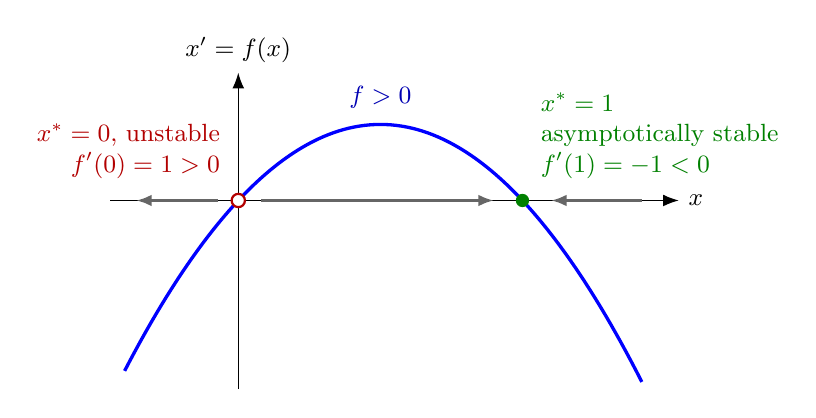
\begin{tikzpicture}[font=\small, >={Latex[length=2mm]}]
  \begin{axis}[width=8.8cm, height=5.6cm, axis lines=middle, axis line style={->},
      xmin=-0.45, xmax=1.55, ymin=-0.62, ymax=0.42, xtick=\empty, ytick=\empty,
      xlabel={$x$}, ylabel={$x'=f(x)$}, xlabel style={anchor=west}, ylabel style={anchor=south},
      tick label style={font=\small}, domain=-0.4:1.42, samples=100, clip=false]
    \addplot[blue, very thick] {x*(1-x)};
    % direction of motion on the phase line
    \draw[->, very thick, gray!80!black] (axis cs:-0.07,0) -- (axis cs:-0.36,0);
    \draw[->, very thick, gray!80!black] (axis cs:0.08,0) -- (axis cs:0.9,0);
    \draw[->, very thick, gray!80!black] (axis cs:1.42,0) -- (axis cs:1.1,0);
    % equilibria
    \draw[red!70!black, thick, fill=white] (axis cs:0,0) circle (2.4pt);
    \fill[green!50!black] (axis cs:1,0) circle (2.4pt);
    \node[red!70!black, anchor=south east, align=right] at (axis cs:-0.03,0.04) {$x^*=0$, unstable\\ $f'(0)=1>0$};
    \node[green!50!black, anchor=south west, align=left] at (axis cs:1.03,0.04) {$x^*=1$\\ asymptotically stable\\ $f'(1)=-1<0$};
    \node[blue!70!black, anchor=south] at (axis cs:0.5,0.27) {$f>0$};
  \end{axis}
\end{tikzpicture}
\end{document}
